% !TEX root = ../main.tex
% chktex-file 46
\def\cgScale{0.6}

\chapter{Wissensgraph\-konstruktion aus Kommunikations\-daten}%
\label{sec:text2kg}

Auf Basis der vorgestellten Konzeptgraphen, CoreNLP und PSL wird im folgenden Kapitel ein Verfahren für die online Konstruktion eines Wissensgraphen aus natürlichsprachlichen Textnachrichten aufgebaut.
Der Fokus liegt dabei primär auf der generellen Architektur des Verfahrens.
Das Resultat ist also als Proof-of-Concept zu verstehen, auf dessen Basis praxistaugliche Systeme konzipiert werden können.

\begin{figure}[h]
	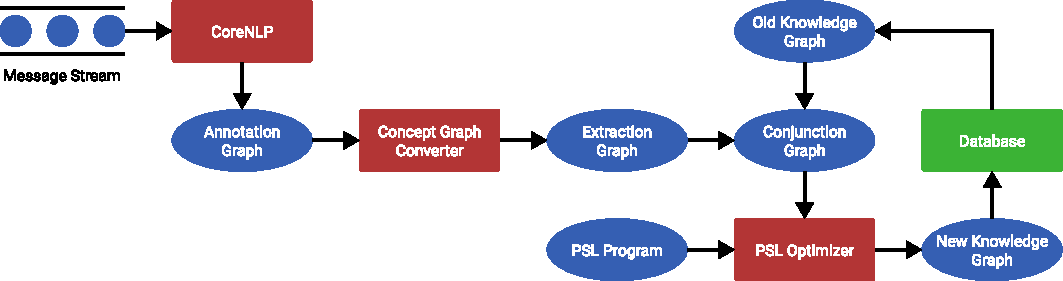
\includegraphics[width=\textwidth]{gfx/text2kg/architecture.pdf}
	\caption{Grobes Architekturdiagramm der Konstruktionspipeline}\label{fig:text2kg:architecture}
\end{figure}
Das im Folgenden vorgestellte Verfahren folgt einem dreistufigen Pipeline-Modell:
\begin{enumerate}
	\item Mittels CoreNLP wird eine eintreffende Textnachricht in einen Abhängigkeitsgraphen transformiert.
	\item Der resultierende Abhängigkeitsgraph wird in einen sog.\ Extraktionsgraphen umgewandelt.
		Hierbei handelt es sich um einen Konzeptgraphen, der den Inhalt der Nachricht formal repräsentiert.
	\item Der Extraktionsgraph wird mit dem bestehenden Wissensgraphen verschmolzen.
		Dies entspricht der Konjunktion der durch die beiden Graphen repräsentierten logischen Ausdrücke.
		Der resultierende Konjunktionsgraph wird als Eingabe für ein PSL-Programm verwendet, welches auf Basis des hinzugekommenen Wissens neue Beziehungen im Wissensgraphen inferiert.
\end{enumerate}
Die Beschreibung dieser Pipeline erfolgt in vier Abschnitten.
\treft{sec:text2kg:ontology} beschreibt die Ontologie der konstruierten Wissensgraphen.
Nachdem beschrieben ist, wie die zu konstruierenden Wissensgraphen strukturell aufgebaut sein sollen, wird schließlich in \treft{sec:text2kg:nlp} und \treft{sec:text2kg:psl} die Transformation von einem Text in einen Extraktionsgraph, bzw.\ von einem Extraktionsgraph in einen Wissensgraph beschrieben.
In \treft{sec:text2kg:implementation} wird abschließend kurz die technische Umsetzung des zuvor beschriebenen Verfahrens erläutert.

\section{Wissensgraphontologie}%
\label{sec:text2kg:ontology}

Bevor Wissensgraphen konstruiert werden können, muss spezifiziert werden, wie diese strukturell aufgebaut sein sollen.
Um komplexe logische Beziehungen ausdrücken zu können, wird die bereits vorgestellte Konzeptgraph-Struktur verwendet.
Dabei bleibt allerdings offen, welche Prädikate vorkommen können und welche Bedeutung sie haben.
Außerdem ist unklar, wie mit Konzeptgraphen modale Aussagen ausgedrückt werden.
Damit aus einem Konzeptgraphen ein Wissensgraph wird, muss eine Ontologie gegeben sein, welche diese offenen Punkte schließt.
Im Folgenden wird beschrieben, wie die in dieser Arbeit verwendete Ontologie aufgebaut ist.

\subsection{Verwendete Prädikate}%
\label{sec:text2kg:ontology:pred}

Im ersten Schritt wird geklärt, welche Prädikate in den konstruierten Wissensgraphen vorkommen können.
Es ist nicht sinnvoll, beliebige Prädikate zuzulassen, da für eine effiziente maschinelle Weiterverarbeitung der Wissensgraphen eine Semantik für alle vorkommenden Prädikate definiert sein muss.
Für die Wissensgraphen in dieser Arbeit wird eine Menge von sechs Prädikaten verwendet.

\paragraph{Syntax}
Bevor diese Prädikate näher erläutert werden, wird allerdings die Konzeptgraphsyntax leicht modifiziert.
Da alle verwendeten Prädikate entweder unär oder binär sein werden, kann eine kompaktere Notation benutzt werden:
\begin{align}
	\vcenter{\hbox{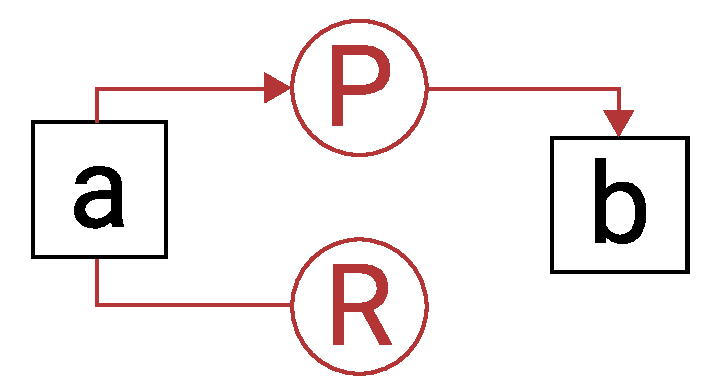
\includegraphics[scale=0.23]{gfx/text2kg/relationNodeAlternativeSyntax1.pdf}}}
	\Leftrightarrow
	\vcenter{\hbox{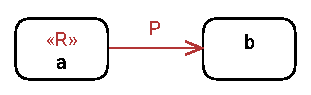
\includegraphics[scale=\cgScale]{gfx/text2kg/relationNodeAlternativeSyntax2.pdf}}}
\end{align}
Relationsknoten werden nicht mehr dargestellt.
Bei unären Relationen werden die Relationsknotenbezeichner stattdessen mit in die Konzeptknoten geschrieben.
Binäre Relationen werden durch eine bezeichnete Kante zwischen dem ersten und zweiten Argument repräsentiert.
Der nun nicht mehr explizit dargestellte Relationsknoten befindet sich dabei implizit im Kontext des kleinsten Arguments gemäß der $\leq$-Ordnung, sodass alle dominierenden Knoten erhalten bleiben.

\paragraph{Wissensmodell}
Um eine semantisch konsistente Menge von Wissensgraph-Prädikaten zu definieren, ist es sinnvoll zuvor ein Modell zu definieren, welches den abstrakten Begriff des \textit{Konzeptes} formalisiert.
Konzepte sind das zentrale Syntaxelement in Konzeptgraphen;
ähnlich wie Variablen in der Prädikatenlogik, haben sie jedoch keine inhärente Bedeutung.

Im Folgenden wird ein Konzept $x$ durch eine Eigenschaftsmenge $prop(x) = \{ p_1, \dots, p_n \}$ spezifiziert.
Alle Konzeptgraph-Relationen von $x$, beschreiben Eigenschaften von $prop(x)$.
Es ist unrealistisch $prop(x)$ mittels Relationen vollständig zu definieren, da dies gleichbedeutend mit einer exakten formalen Beschreibung jedes beliebigen Konzeptes $x$ wäre.
Das Ziel ist daher stattdessen, die Eigenschaftsmengen von Konzepten in Relation zueinander zu beschreiben.
Der Wissensgraph ist also ein Formalismus zur Beschreibung von Eigenschaften der Eigenschaftsmengen von Konzepten.

\paragraph{Prädikate}
Abhängig davon, welche Eigenschaften erfasst werden sollen, können die zu verwendenden Prädikate stark variieren.
Die für diese Arbeit verwendete Prädikatsmenge hat nicht das Ziel der Vollständigkeit, sondern versucht vielmehr einige wesentliche Eigenschaften natürlichsprachlicher Aussagen zu erfassen.
Gemäß dieser Prämisse wurden sechs Wissensgraph-Prädikate definiert.
\begin{enumerate}
	\item \textbf{$label \subseteq \text{concept} \times \text{string}$:}
		Das $label$-Prädikat wird benutzt, um den Bezeichner eines Konzeptes zu repräsentieren.
		Jedes Konzept hat höchstens einen Bezeichner.
		Da Konzepte aus natürlichsprachlichen Texten extrahiert werden, kann i.~d.~R. allen Konzepten ein solcher Bezeichner zugeordnet werden.
		In der bisher verwendeten Konzeptgraphsyntax lassen sich derartige Konstanten allerdings nicht ausdrücken.
		Die Syntax wird daher erneut leicht modifiziert.
		Das $label$ eines Konzeptes wird nun, statt des Variablenbezeichners, in den zugehörigen Konzeptknoten geschrieben.
		\begin{align}
			\vcenter{\hbox{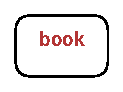
\includegraphics[scale=\cgScale]{gfx/text2kg/label.pdf}}}
			\Leftrightarrow
			\exists\, x: {\color{rot}label(x, \text{``book''})} % chktex 21
		\end{align}
	\item \textbf{$named \subseteq \text{concept}$:}
		Die Bedeutung des durch $label$ beschriebenen Bezeichners kann stark variieren.
		Für die meisten Konzepte ist das $label$ ein Verweis auf ein natürlichsprachliches Wort, dessen Bedeutung übernommen wird.
		Manche Konzepte, wie z.~B. Personen, Städte oder Firmen, lassen sich darüber hinaus jedoch durch ihren Bezeichner identifizieren; diese Konzepte erhalten das Attribut $named$.
	\item \textbf{$inst \subseteq \text{concept}^2$:}
		Die $inst$-Beziehung zwischen Konzepten entspricht grob der \textit{IS-A}-Beziehung semantischer Netze.
		Das Vorhandensein von $inst(x, y)$ impliziert, dass $prop(x) \subseteq prop(y)$ gilt;
		$inst$ ist also reflexiv und transitiv.
		\begin{align*}
			\textit{``the good book''}
			\Rightarrow
			\vcenter{\hbox{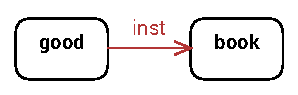
\includegraphics[scale=\cgScale]{gfx/text2kg/inst.pdf}}}
		\end{align*}
	\item \textbf{$relation \subseteq \text{concept}$:}
		Da die Prädikatsmenge eingeschränkt ist, können keine eigenen Prädikate für Worte eingeführt werden, die Konzepte in Relation zueinander setzen (z.~B. \textit{X likes Y}).
		Stattdessen werden sog.\ Relationskonzepte verwendet, d.~h.\ Konzepte, die andere Konzepte zueinander in Beziehung setzen.
		Relationskonzepte $r$ werden durch das unäre Prädikat $relation(r) \Leftrightarrow `relation \in prop(r)$ gekennzeichnet.
		Um die durch $r$ zueinander in Beziehung gesetzten Konzepte zu beschreiben werden die Prädikate $agent$ und $patient$ verwendet.
	\item \textbf{$agent \subseteq \text{concept}^2$:}
		Das $agent$-Prädikat zwischen einem Konzept $x$ und dem sog.\ Agens $y$ wird benutzt, um eine kausale Abhängigkeit des $x$ von $y$ zu beschreiben.
		$agent(x, y) \Leftrightarrow (`cause, y) \in prop(x)$ sagt also aus, dass $x$ aufgrund von $y$ existiert.
	\item \textbf{$patient \subseteq \text{concept}^2$:}
		Der Patiens $y$ eines Konzeptes $x$ ist ein Konzept, dessen Eigenschaften durch $x$ verändert werden.
		Es wird dabei davon ausgegangen, dass $x$ eine Eigenschaft $p_x \in prop(x)$ hat, die beschreibt, wie $x$ andere Konzepte verändert.
		$patient(x, y)$ impliziert, dass $prop(y)$ die durch $p_x$ geforderten Eigenschaften hat.
		$p_x$ lässt sich für natürlichsprachliche Konzepte offensichtlich nicht sinnvoll formal definieren.
		Dies ist allerdings auch nicht notwendig, wenn $p_x$ als mittels $label$ gegebenes Domänenwissen betrachtet wird, welches erst bei der Interpretation der Daten eingebracht wird.
\end{enumerate}
Die Prädikate $agent$ und $patient$ sind grob an die linguistische Idee des Proto-Agens und Proto-Patiens angelehnt~\cite{Dowty1991}.
Zusammen mit den anderen Prädikaten haben sie sich als hinreichend mächtig erwiesen, um eine Vielzahl natürlichsprachlicher Aussagen abzubilden.
\begin{align*}
	\textit{``I saw you yesterday.''}
	\Rightarrow
	\vcenter{\hbox{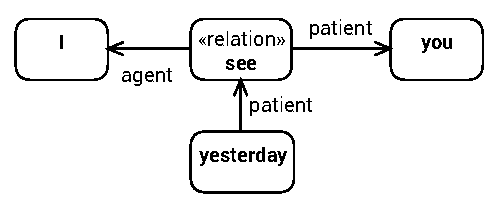
\includegraphics[scale=\cgScale]{gfx/text2kg/relAgPat.pdf}}}
\end{align*}

\subsection{Modale Kontexte}%
\label{sec:text2kg:ontology:modal}

Nachdem nun die verwendeten Prädikate beschrieben wurden, wird im zweiten Schritt geklärt, wie im Wissensgraphen Modalität repräsentiert wird.
Beispiele für modale Aussagen sind:
\begin{center}
	\textit{``I {\color{blau}think} that {\color{rot}the book is good}.''}\\
	\textit{``{\color{rot}I} {\color{blau}don't want} to {\color{rot}see you}.''}
\end{center}
Die beiden Teilaussagen \textit{\color{rot}``the book is good''} und \textit{\color{rot}``I see you''} sind offensichtlich nicht unbedingt wahr, sondern beschreiben Möglichkeiten, die in Abhängigkeit von \textit{\color{blau}think} bzw.\ \textit{\color{blau}don't want} wahr oder falsch werden könnten.
Ob die Aussagen wahr werden, hängt davon ab, inwiefern das Denken oder Wollen einer Person mit der Realität --- auch aktuale Welt genannt --- übereinstimmt.
Dies ist je nach Person stark verschieden; manche tendieren dazu die allgemein als wahr akzeptierten Aussagen zu denken bzw.\ entsprechend ihrer Wünsche zu handeln, andere nicht.

Um derartige Möglichkeiten und Notwendigkeiten direkt zu repräsentieren, reichen die vorgestellten Konzeptgraphen mit Negationskontexten nicht aus.
Sowa hat dieses Problem ebenfalls erkannt und daher weitere Kontexttypen eingeführt.
Die Beschreibung dieser zusätzlichen Kontexttypen ist allerdings oftmals zu unpräzise für eine eindeutige Übersetzung in die Prädikatenlogik.
Aufbauend auf Sowas Ideen wird in dieser Arbeit daher eine Variante modaler Kontexte eingeführt, die die Übersetzbarkeit in die Prädikatenlogik erster Ordnung bewahrt.
Da die zuvor vorgestellten Konzeptgraphen bereits vollständig und korrekt sind, handelt es sich bei diesen modalen Kontexten also lediglich um eine Kurzschreibweise.
Insgesamt gibt es durch die Erweiterung um modale Kontexe nun vier Kontexttypen:
\begin{multicols}{2}
	\flushleft\begin{enumerate}
		\item Positiver Aktualkontext
		\item Negativer Aktualkontext
		\item Positiver Möglichkeitskontext
		\item Negativer Möglichkeitskontext
	\end{enumerate}
\end{multicols}
Die modale Notwendigkeit hat keine eigenen Kontexttypen erhalten, um konsistent zur Quantisierung in Konzeptgraphen zu bleiben.
So, wie der Allquantor in Konzeptgraphen durch Negation der negierten existenzquantisierten Aussage ausgedrückt wird, wird die Notwendigkeit durch Negation der negativen Möglichkeit ausgedrückt.

Da es nun vier Kontexttypen gibt, muss die Konzeptgraphsyntax leicht angepasst werden, um zwischen den verschiedenen Typen differenzieren zu können:
\begin{figure}[h]
	\centering
	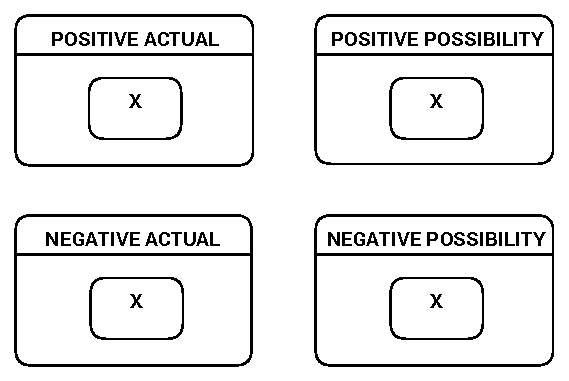
\includegraphics[scale=\cgScale]{gfx/text2kg/contextTypes.pdf}
	\caption{Konzeptgraphsyntax für modale Kontexte}\label{fig:text2kg:contextTypes}
\end{figure}

\paragraph{Positiver Aktualkontext}
Dieser Kontexttyp hat keinen Einfluss auf die Bedeutung der enthaltenen Knoten.
Er entspricht in etwa der Klammerung in der Prädikatenlogik.
Das \textit{Sheet of Assertion}~$\top$ ist ein solcher Kontext, abgesehen davon tauchen positive Aktualkontexte allerdings nicht auf;
sie werden hier lediglich der Vollständigkeit halber erwähnt.
\begin{align}
	\vcenter{\hbox{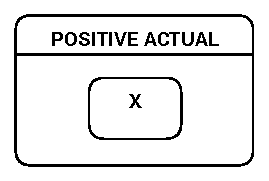
\includegraphics[scale=\cgScale]{gfx/text2kg/positiveActual.pdf}}}
	\Leftrightarrow
	\vcenter{\hbox{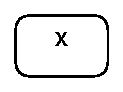
\includegraphics[scale=\cgScale]{gfx/text2kg/x.pdf}}}
	\Leftrightarrow
	\exists x: label(x, \text{``X''})
\end{align}

\paragraph{Negativer Aktualkontext}
Entspricht dem bisherigen Negationskontext.
\begin{align}
	\vcenter{\hbox{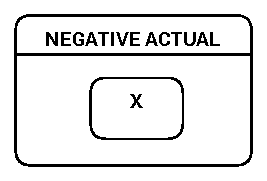
\includegraphics[scale=\cgScale]{gfx/text2kg/negativeActual.pdf}}}
	\Leftrightarrow
	\lnot \exists x: label(x, \text{``X''})
\end{align}

\paragraph{Positiver Möglichkeitskontext}
Dieser Kontexttyp bildet die modale Möglichkeit ab.
Um die Übersetzbarkeit in die Prädikatenlogik beizubehalten, wird hierfür keine fundamental neue Struktur eingeführt.
Es wird stattdessen die Tatsache ausgenutzt, dass sich die modalen Operatoren gemäß der Mögliche-Welten-Interpretation analog zu den prädikatenlogischen Quantoren verhalten.\\
\begin{align*}
	{\color{rot}\square} P(x)\ &\Leftrightarrow \lnot {\color{blau}\lozenge} \lnot P(x) \\
	{\color{rot}\forall} w: world(w) \rightarrow P_w(x)\ &\Leftrightarrow \lnot {\color{blau}\exists} w: world(w) \land \lnot P_w(x) \numberthis
\end{align*}
Die Aussage \textit{``$P(x)$ gilt notwendigerweise''}, wird also als \textit{``Es gibt keine Welt $w$ in der $P_w(x)$ nicht gilt''} aufgefasst.
Statt von Welten, wird in modalen Konzeptgraphen allerdings von Kontexten gesprochen.
\begin{align*}
	\vcenter{\hbox{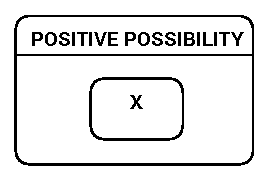
\includegraphics[scale=\cgScale]{gfx/text2kg/positivePossib.pdf}}}
	&\Leftrightarrow
	\vcenter{\hbox{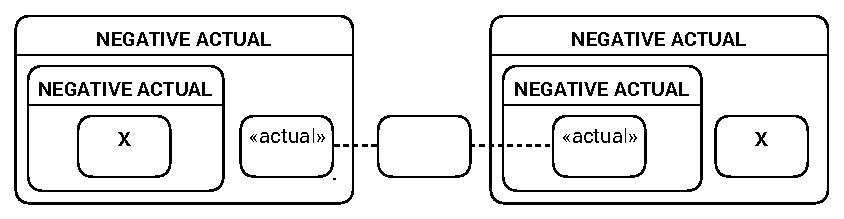
\includegraphics[scale=\cgScale]{gfx/text2kg/possibExpansion.pdf}}} \numberthis \\
	&\Leftrightarrow
	\exists c: context(c) \land (actual(c) \leftrightarrow \exists x: label(x, \text{``X''}))
\end{align*}
Anders als Aktualkontexte tauchen Möglichkeitskontexte explizit in der prädikatenlogischen Repräsentation auf, sie lassen sich also nicht nur als Kontext, sondern zugleich auch als Konzept auffassen.
Der in einem Möglichkeitskontext $c$ enthaltene Teilgraph $G$ ist dabei genau dann wahr, wenn der Kontext die aktuale Welt beschreibt~($\Leftrightarrow actual(c)$).
Solange $actual(c)$ unbekannt ist, kann also keine Aussage über die Wahrheit von $G$ gemacht werden.
Wenn $actual(c)$ jedoch wahr bzw.\ falsch ist, ist $c$ äquivalent zu einem positiven bzw.\ negativen Aktualkontext.

Zur Bestimmung von des Wahrheitswertes von $actual(c)$ ist i.~d.~R. domänenspezifisches Wissen notwendig.
Dieses domänenspezifische Wissen kann durch sog.\ Kontextrelationen eingebracht werden.
Da Möglichkeitskontexte zugleich Konzepte sind, lassen sie sich zu anderen Konzepten in Relation setzen.
Dies ist z.~B. dann nützlich, wenn man die Aussage \textit{``I {\color{blau}think} that {\color{rot}the book is good}.''} repräsentieren möchte.

\begin{align*}
	&\vcenter{\hbox{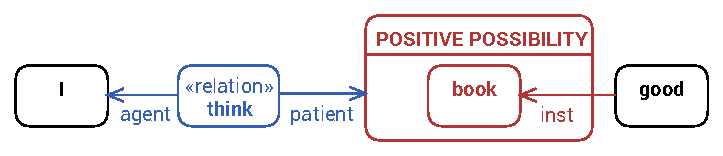
\includegraphics[scale=\cgScale]{gfx/text2kg/possibCtxRelationExample.pdf}}} \numberthis \displaybreak[0]\\
	\Leftrightarrow
	\exists i, g, t, c:&\ label(i, \text{``I''}) \land label(g, \text{``good''}) \\
	\land&\ {\color{blau}label(t, \text{``think''}) \land relation(t) \land agent(t, i) \land patient(t, c)} \\
	\land&\ {\color{rot}context(c) \land (actual(c) \leftrightarrow \exists b: label(b, \text{``book''}) \land inst(g, b))}
\end{align*}
Durch die Verknüpfung $patient(t, c)$ eines Konzeptes mit einem Kontext kann Wissen über das Konzept benutzt werden, um Schlüsse über die Aktualität des Kontextes zu ziehen.
Wie dies ablaufen kann, wird im Rahmen dieser Arbeit nicht beschrieben~\tref{sec:conclusion:todo}.

\paragraph{Negativer Möglichkeitskontext}
Lediglich eine Kurzschreibweise für einen positiven Möglichkeitskontext der einen negativen Aktualkontext umgibt.
\begin{align}
	\vcenter{\hbox{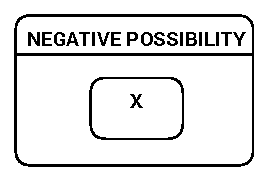
\includegraphics[scale=\cgScale]{gfx/text2kg/negativePossib.pdf}}}
	\Leftrightarrow
	\vcenter{\hbox{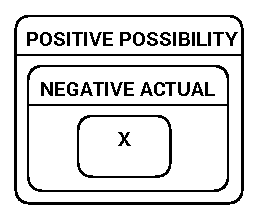
\includegraphics[scale=\cgScale]{gfx/text2kg/negativePossibExpansion.pdf}}}
\end{align}

\section{NLP-Phase}%
\label{sec:text2kg:nlp}

In diesem Abschnitt werden die ersten beiden Stufen der Konstruktionspipeline beschrieben.
Die erste Stufe ist im Wesentlichen lediglich ein Wrapper um verschiedene CoreNLP-Annotatoren.
In der zweiten Stufe werden dann die CoreNLP-Annotationen in eine Konzeptgraphinstanz der in~\ref{sec:text2kg:ontology} beschriebenen Ontologie transformiert.
\begin{figure}[h]
	\centering
	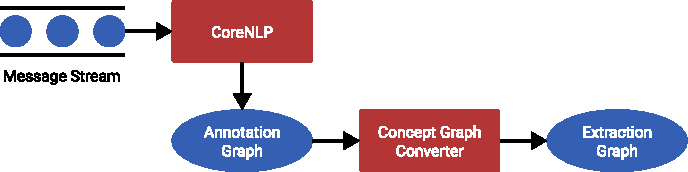
\includegraphics[width=0.67\textwidth]{gfx/text2kg/nlpPhase.pdf}
	\caption{NLP-Phase der Konstruktionspipeline}\label{fig:text2kg:nlpPhase}
\end{figure}

\subsection{Nachrichtenformat}%
\label{sec:text2kg:nlp:msg}

Vor der Beschreibung der Pipeline-Stufen muss geklärt werden, wie die eingegebenen Nachrichten aufgebaut sind.
Da diese Arbeit lediglich die grundlegende Architektur eines Wissensgraph-Konstruktionsverfahrens beschreibt, wurde eine vereinfachte Struktur gewählt, die die wesentlichen Eigenschaften von Nachrichten enthält.
Eine Nachricht wird daher im Folgenden als ein Tupel mit den folgenden Komponenten verstanden:
\begin{enumerate}
	\item \textbf{Sender:}
		Als Sender wird, der Einfachheit halber, der Name des Absenders verwendet.
		Im Kontext von E-Mail Nachrichten müsste zwar zwischen dem Absendernamen und der Absenderadresse differenziert werden, diese Unterscheidung macht das Verfahren allerdings komplizierter, ohne dabei die Kernaspekte zu bereichern.
	\item \textbf{Empfänger:}
		Auch hier wird lediglich der Empfängername benutzt.
		Nachrichten mit mehreren Empfängern werden in dieser Arbeit nicht betrachtet.
	\item \textbf{Sendezeit:}
		Gemeint ist hiermit ein Datum oder Zeitpunkt im TIMEX3-Format~\cite{TIMEX3} (z.~B. \texttt{YYYY-MM-DD}), welches den Absendezeitpunkt der Nachricht beschreibt.
		TIMEX3 unterstützt höchstens sekundengenaue Angaben und keine Zeitzonen.
		Für die Zwecke dieser Arbeit sind diese Einschränkungen allerdings nicht problematisch.
	\item \textbf{Inhalt:}
		Der Nachrichteninhalt wird als natürlichsprachliche Zeichenkette verstanden.
		Als Sprache wird dabei Englisch angenommen, da CoreNLP dann die besten Ergebnisse liefert.
		Zudem werden eingebundene Multimedia-Inhalte und Anhänge nicht berücksichtigt.
\end{enumerate}

Zwei sehr einfache exemplarische Nachrichten sind:
\begin{center}\pbox{\textwidth}{
	$(m_1)$ \texttt{2017-06-11}: Bob $\rightarrow$ Alice: \textit{``I think I saw you in the red tent today.''} \\ % chktex 8
	$(m_2)$ \texttt{2017-06-12}: Alice $\rightarrow$ Bob: \textit{``Oh\dots I don't remember seeing you yesterday.''} % chktex 8
}\end{center}

\subsection{CoreNLP Annotation}%
\label{sec:text2kg:nlp:corenlp}

In \treft{sec:theory:nlp} wurden die für diese Arbeit wesentlichen Annotatoren bereits vorgestellt: Tokenization, Lemmatization, POS-Tagging, NER, Coreference Resolution und Dependency Parsing.
Um mit den Ergebnissen all dieser Annotatoren zu arbeiten, werden jene in einer gemeinsamen Datenstruktur zusammengefasst, dem sog.\ \textit{Annotations\-graphen}.
Hierbei handelt es sich um den Abhängigkeitsgraphen des CoreNLP \textit{Enhanced\texttt{++} Dependency Parsers}, in den die Ergebnisse der anderen Annotatoren eingefügt wurden:
\begin{enumerate}
	\item \textbf{Lemmata:}
		Die Vollformen der Token werden durch ihre Lemmata ersetzt.
		Dieser Änderung liegt die Annahme zugrunde, dass die syntaktische Repräsentation einer Wortbeugung i.~d.~R. nicht relevant ist.
		Durch die Lemmatisierung wird es einfacher ähnliche Begriffe aufgrund ihrer textuellen Ähnlichkeit zu identifizieren.
	\item \textbf{POS-Tags:}
		Durch das Verwerfen der Token-Vollformen können wertvolle grammatikalische Informationen verloren gehen.
		Daher wird jedem Token-Knoten sein POS-Tag hinzugefügt, welcher die Wortart und Beugung jedes lemmatisierten Tokens einheitlich repräsentiert.
	\item \textbf{NER-Klassen:}
		Alle Token-Knoten, die der NER-Annotator klassifizieren konnte, erhalten ihre Klasse.
		Für alle von SUTime erkannten Zeitangaben wird zudem ein neuer Knoten eingefügt.
		Alle Token, die an der Spezifikation einer Zeitangabe beteiligt sind (z.~B. \textit{yesterday} und \textit{morning}), werden mittels einer Koreferenzkante mit dem hinzugefügten Zeitknoten verknüpft.
	\item \textbf{Koreferenzklassen:}
		Jede gefundene Token-Koreferenzklasse $C = \{t_1, \dots, t_n\}$ wird als eine Menge von Koreferenzkanten in den Annotatinsgraphen eingefügt.
		Als Kantenmenge wird allerdings nicht $C \times C$ verwendet, da diese unnötig groß ist und zudem nicht alle verfügbaren Informationen repräsentiert.
		Die CoreNLP Coreference Resolution ordnet jeder Klasse nämlich eine sog.\ \textit{Representative Mention} $rep(C) \in C$ zu.
		$rep(C)$ ist das Token einer Klasse, welches diese am besten repräsentiert.
		\begin{align*}
			\text{T}\tikzmark{toma}\text{om is calling hi}\tikzmark{tomb}\text{s brother.}
			\begin{tikzpicture}[overlay,remember picture]
				\draw[-,shorten >=3pt,shorten <=3pt] (toma.center) to[bend right] (tomb.center);
			\end{tikzpicture}
			\Rightarrow
			C = \{\text{Tom}, \text{his}\}, rep(C) = \text{Tom}
		\end{align*}
		Um die $rep$-Information zu erhalten, werden nur Koreferenzkanten von den anderen Klassentoken $C \setminus \{rep(C)\}$ zu $rep(C)$ hinzugefügt.
\end{enumerate}

\figreft{fig:text2kg:annotationGraph1} zeigt den Annotationsgraphen der Beispielnachricht $m_2$.
In den Knoten sind die Token-Lemmata, die NER-Klasse und der POS-Tag dargestellt.
Informationen, die nicht aus dem Abhängigkeitsgraphen stammen, wurden farblich hervorgehoben.
\begin{figure}[h]
	\centering
	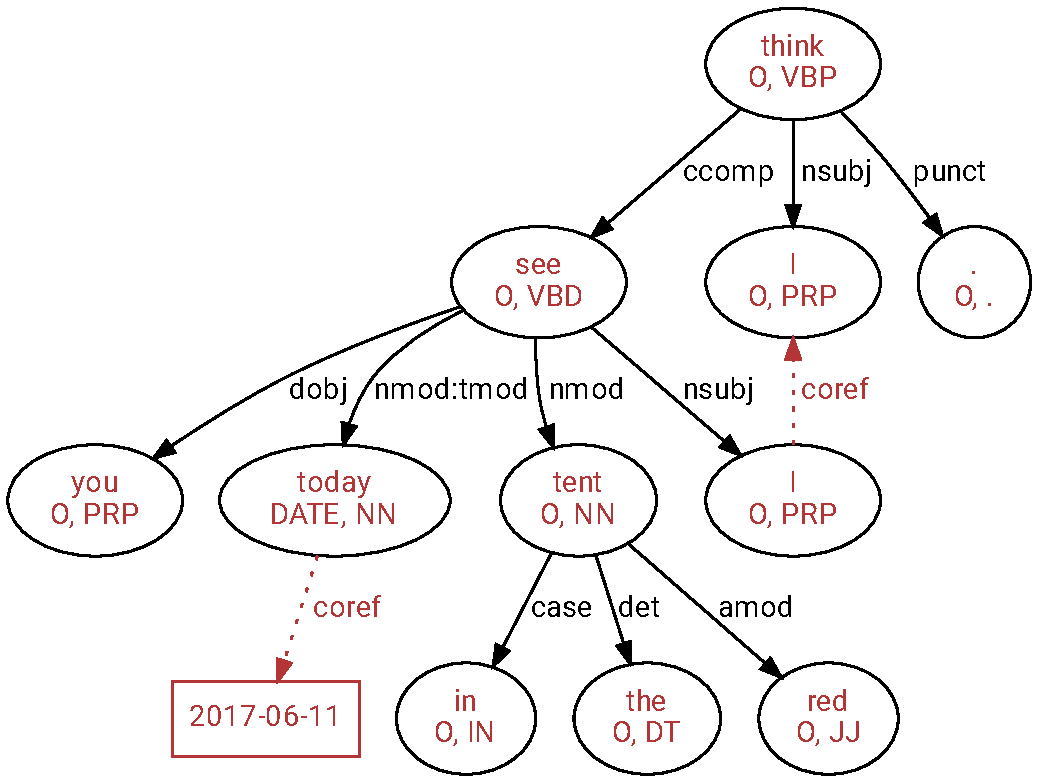
\includegraphics[width=0.6\textwidth]{gfx/text2kg/annotationGraph1.pdf}
	\caption{Annotationsgraph der Nachricht \textit{``I think I saw you in the red tent today.''} vom \texttt{2017-06-11}.}\label{fig:text2kg:annotationGraph1} % chktex 8
\end{figure}

\subsection{Konzeptgraphtransformation}%
\label{sec:text2kg:nlp:transform}

Aus dem Annotationsgraphen einer Nachricht muss im nächsten Schritt der sog.\ \textit{Extraktionsgraph} erstellt werden.
Hierbei handelt es sich um einen Konzeptgraphen mit der in~\ref{sec:text2kg:ontology} beschriebenen Ontologie, der den Inhalt der Nachricht beschreibt.
Da natürliche Sprachen eine höhere Ausdrucksstärke als die Prädikatenlogik erster Ordnung und somit auch als Konzeptgraphen haben, ist es generell unmöglich, jede beliebige Aussage im Extraktionsgraphen zu repräsentieren.
Das Ziel der Extraktionsgraph-Konstruktion ist daher lediglich, einige wesentliche repräsentierbare semantische Strukturen zu identifizieren.

Hierfür wird eine deterministische regelbasierte Transformationspipeline benutzt.
Diese basiert auf der Annahme, dass bestimmte Muster von POS-Tags und grammatikalischen Abhängigkeiten Rückschlüsse auf die semantischen Rollen in einer Aussage zulassen.
Es wird also wenig bis gar kein Wissen über Wortbedeutungen o.~ä.\ verwendet.
Die Transformationspipeline, die im Rahmen dieser Arbeit entwickelt wurde, lässt sich in vier Phasen gliedern.

\begin{figure}[h]
	\centering
	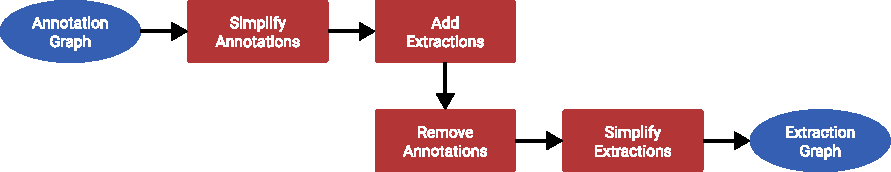
\includegraphics[width=0.84\textwidth]{gfx/text2kg/transformationPipeline.pdf}
	\caption{Annotationsgraph $\rightarrow$ Extraktionsgraph Transformationspipeline}\label{fig:text2kg:transformationPipeline}
\end{figure}
Die einzelnen Transformationsschritte in jeder Phase sind primär exemplarisch zu verstehen.
Um die Extraktionsqualität zu verbessern, können und sollten weitere Schritte hinzugefügt werden.

\subsubsection{1. Phase: Vereinfachen der Annotationen}
In dieser Phase werden im ersten Schritt alle Daten aus dem Annotationsgraphen entfernt, die kein potentieller Bestandteil eines Konzeptes sind (z.~B. Token für Satz- und Sonderzeichen, sowie Interjektionen, wie \textit{``Oh''}).
Die entfernten Token können zwar die Konnotation anderer Token beeinflussen, da deren Übersetzung in Konzeptgraphkonstrukte allerdings ein nicht triviales Problem ist, werden sie hier der Einfachheit halber ignoriert.
Anschließend werden Token, die Bestandteile eines Kompositums sind, zu einem Knoten zusammengefasst, dessen Label die Konkatenation der Lemmata der zusammengefassten Token ist.
Die übrigbleibende Menge von Token-Knoten und Komposita bildet nun die Menge der Konzeptknoten des Wissensgraphen.

\subsubsection{2. Phase: Einfügen der Extraktionen}
Diese Phase ist für das Finden der Konzeptgraphstruktur verantwortlich.
In ihr werden Konzeptgraph-Relationen zwischen den Konzept- bzw. Token-Knoten aus der ersten Phase und Kontexte in den Annotationsgraphen eingefügt.

\paragraph{Einfügen von $label$- und $named$-Prädikaten}
Das Einfügen der Bezeichner ist trivial.
Als $label$ wird für alle Konzepte ihr Lemma verwendet.
Alle Konzepte mit einem POS-Tag, der einen Eigennamen impliziert (\texttt{NNP} und \texttt{NNPS}), erhalten das $named$-Attribut.

\paragraph{Einfügen von $relation$-, $agent$- und $patient$-Prädikaten}
Agens- und Patiens-Relationen bilden einen Großteil der semantischen Beziehungen im Wissensgraphen ab.
Sie werden auf drei Wegen aus den Annotationen extrahiert.
\begin{itemize}
	\item \textbf{Prädikate:}
		Ein recht offensichtlicher Ansatz ist das Nutzen von Subjekt- und Objekt-Beziehungen.
		Direkte Objekte eines Prädikates sind i.~d.~R. auch dessen Patiens.
		Bei Subjekten ist die Diathese des Prädikates zu beachten.
		In Aktiv-Konstruktionen entspricht das Subjekt für gewöhnlich dem Agens.
		Bei passiven Prädikaten hingegen, ist das Subjekt der Patiens.
		Prädikate können dabei meist als $relation$ aufgefasst werden.
		\begin{align*}
			\text{Ali}\tikzmark{alice}\text{ce}\ %
			{\color{rot}\overbrace{\text{\color{black}visi}\tikzmark{visited}\text{\color{black}ted}}^{relation}}\ %
			\text{Bo}\tikzmark{bob1}\text{b. H}\tikzmark{bob2}\text{e was being}\ %
			{\color{rot}\overbrace{\text{\color{black}interv}\tikzmark{interviewed}\text{\color{black}iewed.}}^{relation}}
			\begin{tikzpicture}[overlay,remember picture]
				\draw[->,rot,shorten >=3pt,shorten <=3pt] (visited.center) to[bend left] node[below] {\color{rot}$\scriptstyle agent$} (alice.center);
				\draw[->,rot,shorten >=3pt,shorten <=3pt] (visited.center) to[bend right] node[below] {\color{rot}$\scriptstyle patient$} (bob1.center);
				\draw[->,rot,shorten >=3pt,shorten <=3pt] (interviewed.center) to[bend left] node[below] {\color{rot}$\scriptstyle patient$} (bob2.center);
			\end{tikzpicture}
		\end{align*}

		Eine Ausnahme der vorigen Regeln sind Kopulae, da sie keine konkrete Eigen\-bedeutung haben und somit auch keinen Patiens haben können, den sie verändern.
		Es handelt sich stattdessen um Bindewörter, die ihrem Subjekt die Eigenschaften ihres Objekts zuschreiben.
		Da CoreNLP Kopulae erkennt, lässt sich diese Ausnahme leicht umsetzen.
		Im Englischen ist die Erkennung relativ trivial, da nur das Verb \textit{to be} Kopula ist.
		Der Umgang mit Kopulae wird im Kontext der $inst$-Relation betrachtet.

		Konkret werden also folgende Transformationen durchgeführt:
		$nsubj(x, y) \rightarrow agent(x, y)$, $nsubjpass(x, y) \lor dobj(x, y) \rightarrow patient(x, y)$ und $tag(x, \text{VB*}) \rightarrow relation(x)$.
		Dabei darf $x$ keine Kopula sein.
	\item \textbf{Präpositionen:}
		Neben Prädikaten werden Präpositionen häufig zum Verknüpfen von Konzepten benutzt.
		Diese haben im Gegensatz zu Prädikaten jedoch im Allgemeinen keinen Agens.
		Stattdessen lässt sich das auf eine Präposition $p$ folgende Konzept $x$ als Patiens von $p$ auffassen.
		Wird nun eine solche Präpositionalkonstruktion in Beziehung zu einem anderen Konzept $y$ gesetzt, wird $y$ von $x$ verändert, $y$ ist dann also Patiens von $x$.\\
		\begin{align*}
			\text{The pen fe}\tikzmark{fell}\text{ll bel}\tikzmark{below2}\text{ow the ch}\tikzmark{chair2}\text{air.}
			\begin{tikzpicture}[overlay,remember picture]
				\draw[->,rot,shorten >=3pt,shorten <=3pt] (below2.center) to[bend right] node[below] {\color{rot}$\scriptstyle patient$} (chair2.center);
				\draw[->,rot,shorten >=3pt,shorten <=3pt] ([yshift=5pt] chair2.north) to[bend right] node[above=-3pt] {\color{rot}$\scriptstyle patient$} ([yshift=5pt] fell.north);
			\end{tikzpicture}
		\end{align*}

		Konkret wird die folgende Transformation durchgeführt:
		\[nmod(x, y) \lor nummod(x, y) \lor case(x, y) \rightarrow patient(y, x)\]
	\item \textbf{Adverbien:}
		$advmod(x, y) \rightarrow patient(y, x)$, da die Veränderung eines Verbs durch ein Adverb ebenfalls als eine Patiens-Beziehung aufgefasst werden kann.
\end{itemize}

\paragraph{Einfügen von $inst$-Prädikaten}
Für die Bestimmung von $inst$-Relationen werden drei Verfahren benutzt.
\begin{itemize}
	\item \textbf{NER-Klassen:}
		Manche Konzepte besitzen NER-Klassen (z.~B. Person, Ort, Organisation etc.), die bereits $inst$-Relationen abbilden.
		Es werden daher Konzeptknoten für alle vorkommenden Klassen hinzugefügt.
		Diese werden durch $inst$-Kanten mit ihren Instanzen verbunden.
		Die eingefügten Klassenknoten repräsentieren die abstrakten Konzepte der verschiedenen Klassen;
		sie werden also durch ihr $label$ eindeutig identifiziert und erhalten daher das $named$-Attribut.
	\item \textbf{Kopulae:}
		Ein Prädikat, welches Kopula ist, wurde für das Identifizieren von $agent$- und $patient$-Relationen zuvor explizit ausgeschlossen.
		Dies liegt daran, dass Kopulae ihre Subjekte und Objekte i.~d.~R. in ein $inst$-ähnliches Verhältnis setzen.
		\begin{align*}
			\text{Ali}\tikzmark{alice2}\text{ce is tir}\tikzmark{tired}\text{ed.}
			\begin{tikzpicture}[overlay,remember picture]
				\draw[->,rot,shorten >=3pt,shorten <=3pt] (tired.center) to[bend left] node[below] {\color{rot}$\scriptstyle inst$} (alice2.center);
			\end{tikzpicture}
		\end{align*}
		Konkret wird folgende Transformation durchgeführt:
		\[(\exists z: cop(x, z)) \land nsubj(x, y) \rightarrow inst(x, y)\]
	\item \textbf{Attribute und Appositionen:}
		Ähnlich wie Kopulae drücken diese zwei grammatikalischen Beziehungen ein $inst$-ähnliches Verhältnis aus.
		\begin{align*}
			\text{Bo}\tikzmark{bob2}\text{b, a profes}\tikzmark{professional}\text{sional athl}\tikzmark{athlete}\text{ete, runs.}
			\begin{tikzpicture}[overlay,remember picture]
				\draw[->,rot,shorten >=3pt,shorten <=3pt] (athlete.center) to[bend left] node[below] {\color{rot}$\scriptstyle inst$} (bob2.center);
				\draw[->,rot,shorten >=3pt,shorten <=3pt] ([yshift=5pt] professional.north) to[bend left] node[above=-2pt] {\color{rot}$\scriptstyle inst$} ([yshift=5pt] athlete.north);
			\end{tikzpicture}
		\end{align*}
		Die Transformationsregel ist:
		\[amod(x, y) \lor appos(x, y) \rightarrow inst(y, x)\]
\end{itemize}

\paragraph{Einfügen von Kontexten}
Nachdem nun beschrieben wurde, wie die Konzeptgraph-Relationen ermittelt werden, muss noch geklärt werden, wie die Kontexthierarchie aufgebaut wird.
Das gewählte Verfahren lässt sich in zwei Schritte gliedern.
Im ersten Schritt werden ausschließlich positive Möglichkeitskontexte eingefügt.
Im zweiten Schritt werden dann die negativen Aktualkontexte hinzugefügt.
\begin{enumerate}
	\item \textbf{Möglichkeitskontexte:}
		Um Möglichkeitskontexte einfügen zu können, muss zuerst definiert werden, was als Möglichkeit verstanden wird.
		Sowas Ansatz hierfür ist es, Teilsätze (im Englischen \textit{clause} genannt) als solche zu interpretieren, da sie jeweils genau einen Sachverhalt ausdrücken, der möglicherweise wahr ist~\cite[Abschnitt 5.4]{Harmelen2007}.
		Teilsätze können prinzipiell beliebig geschachtelt werden und hängen i.~d.~R. von einem einleitenden Konzept ab;
		sie lassen sich also gut durch entsprechend geschachtelte Möglichkeitskontexte repräsentieren.
		\begin{figure}[t]
			\centering
			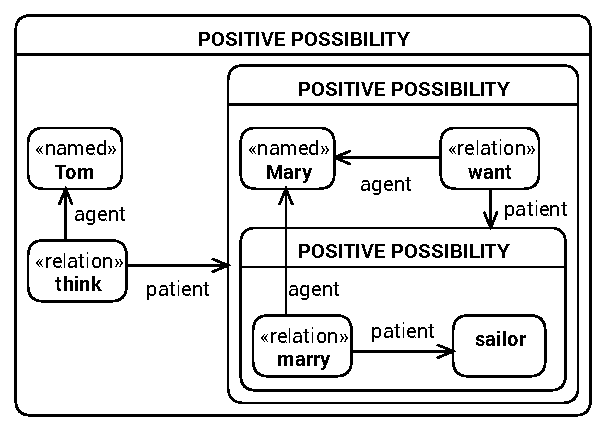
\includegraphics[scale=\cgScale]{gfx/text2kg/contextExtractionGraph1.pdf}
			\caption{\textit{Clause}-basierte Kontextschachtelung der Aussage \textit{``Tom thinks that Mary wants to marry a sailor.''}}\label{fig:text2kg:contextExtractionGraph1} % chktex 8
		\end{figure}
		In dieser Arbeit werden die Möglichkeitskontexte nach dem selben Prinzip eingefügt.
		Teilsätze lassen sich im Annotationsgraphen über die Abhängigkeiten $csubj, ccomp$ und $xcomp$ leicht identifizieren.
		Da der Abhängigkeitsgraph ein DAG ist, können Konzepte in mehreren Teilsätzen bzw. Kontexten auftauchen;
		in diesem Fall muss das Konzept in den kleinsten gemeinsamen umgebenden Kontext (gemäß $\leq$-Relation) eingefügt werden.

		Da die Gesamtheit einer Nachricht $m$ nicht unbedingt wahr sein muss, wird zudem ein Wurzel-Möglichkeitskontext eingefügt, der alle Konzepte, die innerhalb von $m$ erwähnt wurden, enthält.
		Konzeptknoten, die für NER-Klassen eingefügt wurden, fallen nicht darunter, da die Existenz der NER-Klassen, unabhängig vom Inhalt einer Nachricht, als wahr vorausgesetzt wird.

	\item \textbf{Negative Aktualkontexte:}
		Das Formalisieren von Negation in natürlichen Sprachen ist nicht immer eindeutig möglich.
		Dies liegt daran, dass die Bedeutung einer Negation variieren kann; so ist die doppelte Verneinung im Englischen z.~B. manchmal ein umgangssprachliches stilistisches Mittel zur Betonung der Negation (z.~B. \textit{``We don't have no time.''}).
		Da eine umfassende Behandlung aller möglichen Interpretationen der Negation den Rahmen dieser Arbeit gesprengt hätte, wird stattdessen ein stark vereinfachtes Modell verwendet, welches für viele, jedoch nicht für alle Aussagen korrekte Ergebnisse liefert.

		Natürlichsprachliche Negation wird im Folgenden immer als äquivalent zur logischen Negation verstanden.
		Um diese Negationen durch Kontexte zu repräsentieren, muss definiert werden, welche Konzepte durch das Vorkommen einer natürlichsprachlichen Negation betroffen sind.
		Als allgemeine Regel wird benutzt, dass für $agent$ und $patient$-Beziehungen von $x$ nach $y$ die Eigenschaft $x \leq y$~\tref{sec:theory:cg:definition} gilt; d.~h.\ die Nicht-Existenz des Agens oder Patiens eines Prädikates, impliziert dessen Nicht-Existenz.
		\begin{align*}
			\textit{No man helped.}
			\Rightarrow
			\begin{cases}
				{\color{rot}\exists\, helped\ \lnot \exists\, man: agent(helped, man)} & \text{\textit{man} betont}\\ % chktex 21
				{\color{gruen}\lnot \exists\, man\ \exists\, helped: agent(helped, man)} & \text{\textit{helped} betont}\ \checkmark % chktex 21
			\end{cases}
		\end{align*}\\
		Wie das obige Beispiel zeigt, ist diese Regel nicht unbedingt korrekt.
		Die Interpretation gemäß der Regel ist allerdings meist zutreffend, da alternative Interpretationen im Englischen i.~d.~R. nur durch Betonung bestimmter Wörter ausgedrückt werden können.
		Das Einfügen negativer Kontexte läuft gemäß der vorigen Überlegungen wie folgt ab:
		\begin{enumerate}[label*={\arabic*}]
			\item Konzepte, die eine ungerade Anzahl von $neg$-Beziehungen zu Negations-Token haben, werden von einem negativen Aktualkontext umschlossen.
				\begin{align*}
					\textit{No man drinks no beer.}
					\rightarrow
					\vcenter{\hbox{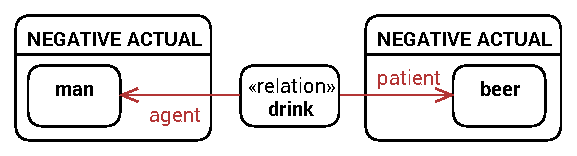
\includegraphics[scale=\cgScale]{gfx/text2kg/negContext1.pdf}}}
				\end{align*}
			\item Es kann nun $agent$- oder $patient$-Kanten geben, die in einen der hinzugefügten Negationskontexe hineinlaufen, was gemäß der vorigen Überlegungen {\color{rot}unzulässig} ist.
				Für jede dieser Kanten von $x$ nach $y$ werden nun Korrekturen vorgenommen, sodass hinterher $x \leq y$ gilt und somit keine Regel-Verletzungen mehr vorliegen.
				Es werden dabei zuerst $patient$-Kanten, dann $agent$-Kanten, korrigiert.
				\begin{enumerate}[label*={.\arabic*}]
					\item Falls vor der Korrektur $y \leq x$ gilt, wird $x$ in den Kontext von $y$ bewegt.
						\begin{align*}
							\vcenter{\hbox{\hspace{-1.4em}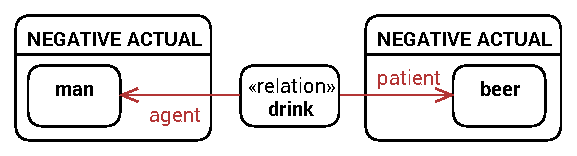
\includegraphics[scale=\cgScale]{gfx/text2kg/negContext1.pdf}}}
							\rightarrow
							\vcenter{\hbox{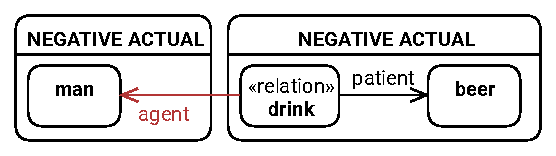
\includegraphics[scale=\cgScale]{gfx/text2kg/negContext2.pdf}}}
						\end{align*}
					\item Andernfalls wird der größte umgebende Kontext von $x$, der nicht $x$ und $y$ umgibt, in den Elternkontext von $y$ verschoben.
					\begin{align*}
						\vcenter{\hbox{\hspace{-0.6em}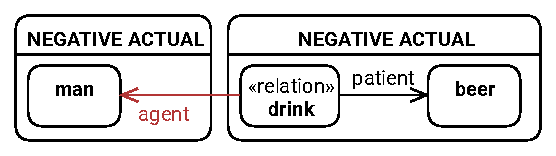
\includegraphics[scale=\cgScale]{gfx/text2kg/negContext2.pdf}}}
						\rightarrow
						\vcenter{\hbox{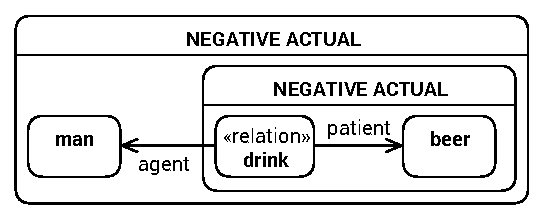
\includegraphics[scale=\cgScale]{gfx/text2kg/negContext3.pdf}}}
					\end{align*}
				\end{enumerate}
		\end{enumerate}
\end{enumerate}

\subsubsection{3. Phase: Entfernen der Annotationen}

Dies ist die trivialste der vier Phasen.
Sie wird hier lediglich der Vollständigkeit halber erwähnt.
Alle Abhängigkeitsgraph-Kanten, sowie POS-Tags und NER-Klassen-Tags werden entfernt, $\mathit{coref}$-Kanten bleiben erhalten.
Das Ergebnis ist nun bereits beinahe ein Konzeptgraph.

\subsubsection{4. Phase: Vereinfachen der Extraktionen}

\paragraph{Koreferenzkanten}
Nach der dritten Phase liegt zwar prinzipiell eine Konzeptgraphstruktur vor, es kann allerdings noch Verletzungen der Eigenschaft dominierender Knoten geben.
Konkret liegt dies daran, dass die in~\ref{sec:text2kg:nlp:corenlp} eingefügten Koreferenzkanten nach Einfügen der Kontexte in benachbarten Kontexten liegen können.
Dies passiert z.~B. dann, wenn in zwei Nebensätzen von derselben Person gesprochen wird, diese jedoch im Hauptsatz nicht auftaucht.
Die Existenz einer derartigen Koreferenz impliziert, dass das koreferente Konzept auch im Kontext des Hauptsatzes existent sein muss, obwohl es nicht explizit erwähnt wird.

Um dominierende Knoten zu erhalten, können die koreferenten Konzepte zu einem Konzeptknoten zusammengefasst werden.
Dieser neue Knoten übernimmt das $label$ der \textit{Representative Mention}~\tref{sec:text2kg:nlp:corenlp} und wird in den kleinsten gemeinsamen umgebenden Kontext aller zusammengefassten Knoten (gemäß der $\leq$-Relation) eingefügt.
Dabei geht zwar die Information verloren, wo und mit welchen Pronomina das Konzept innerhalb der Nachricht referenziert wurde, dies ist allerdings i.~d.~R. irrelevant für die weitere Verarbeitung.
Nach diesem Schritt liegt ein Konzeptgraph vor.

\paragraph{Kontexte}
Um einen möglichst kompakten Konzeptgraphen zu erhalten, werden im letzten Schritt geschachtelte Kontexte vereinfacht.
Dabei werden $2n$-fach geschachtelte Ketten negativer Aktualkontexte entfernt.
Zudem werden positive und negative Möglichkeitskontexte, die lediglich einen negativen Aktualkontext enthalten, zu negativen bzw.\ positiven Möglichkeitskontexten.
Diese Vereinfachungen werden so lange greedy durchgeführt, bis keine weiteren mehr möglich sind.
Das Ergebnis ist der Extraktionsgraph.

\begin{figure}[h]
	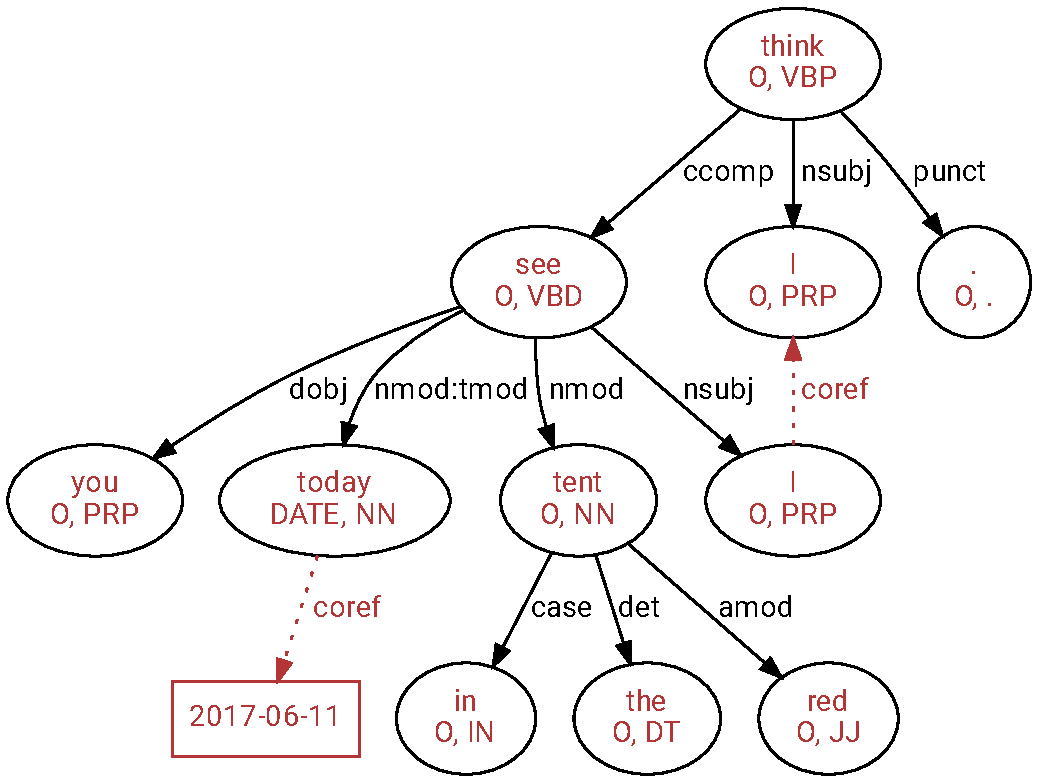
\includegraphics[width=0.4\textwidth]{gfx/text2kg/annotationGraph1.pdf}
	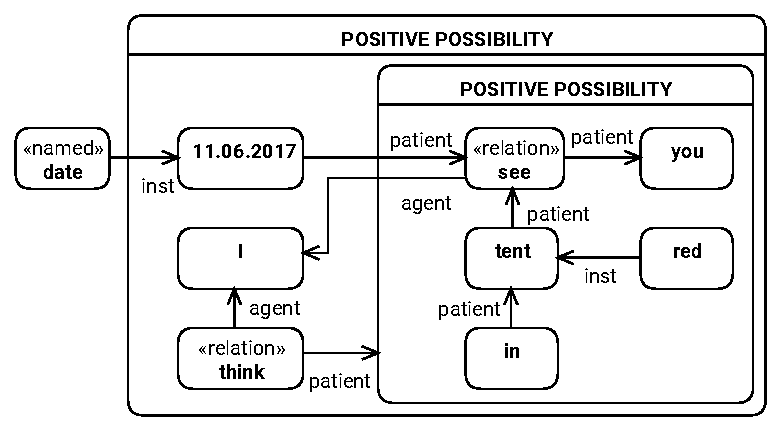
\includegraphics[width=0.6\textwidth]{gfx/text2kg/extractionGraph1.pdf}
	\caption{Annotationsgraph und daraus konstruierter Extraktionsgraph der Nachricht \textit{``I think I saw you in the red tent today.''} vom \texttt{2017-06-11}.}\label{fig:text2kg:extractionGraph1} % chktex 8
\end{figure}

\section{Wissensgraph-Konstruktionsphase}%
\label{sec:text2kg:psl}

Nachdem nun geklärt ist, wie die Konstruktion des Extraktionsgraphen einer Nachricht abläuft, wird im Folgenden beschrieben, wie dieser Extraktionsgraph mittels PSL in einen bestehenden Wissensgraphen eingefügt wird.

\begin{figure}[h]
	\centering
	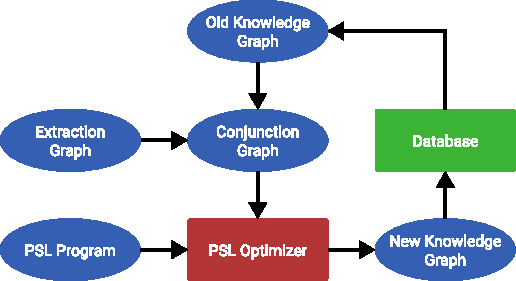
\includegraphics[width=0.49\textwidth]{gfx/text2kg/pslPhase.pdf}
	\caption{Wissensgraph-Konstruktionsphase der Konstruktionspipeline}\label{fig:text2kg:pslPhase}
\end{figure}

\subsection{Konstruktion des Konjunktionsgraphen}%
\label{sec:text2kg:psl:conj}

Der erste Schritt der Wissensgraph-Konstruktion ist das Bilden des sog.\ Konjunktionsgraphen.
Der Konjunktionsgraph ist ein Konzeptgraph, der alle Informationen der einzufügenden Nachricht und des bestehenden Wissensgraphen enthält, allerdings noch keine Schlussfolgerungen aus den hinzugekommenen Informationen beinhaltet.
Der Konjunktionsgraph wird in vier Schritten konstruiert.
\begin{enumerate}
	\item \textbf{Latente Konzepte:}
		Da mit PSL keine neuen Konzepte, sondern lediglich Relationen zwischen gegebenen Konzepten inferiert werden können, müssen alle potentiell möglichen Konzepte bereits im Konjunktionsgraphen vorhanden sein.
		Alle Konzepte des Extraktionsgraphen, die sich innerhalb des Wurzel-Möglichkeitskontextes befinden, werden daher dupliziert und als globale latente Konzepte in das Sheet of Assertion eingefügt.
		Zwischen den latenten Konzepten und den zugehörigen Konzepten werden zudem $inst$-Relationen eingefügt.
		Während der PSL-Inferenz wird dann bestimmt, ob ein latentes Konzept auch außerhalb des Möglichkeitskontextes, aus dem es stammt, existent ist und somit zu einem Konzept wird.
		Da latente Konzepte das durch ihr $label$ repräsentierte Konzept repräsentieren, erhalten sie das $named$-Attribut.
		\begin{align*}
			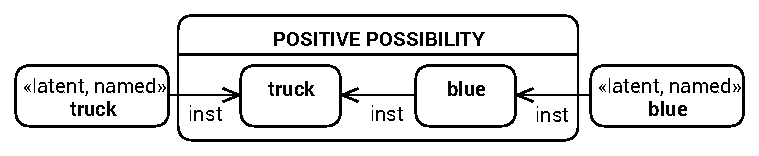
\includegraphics[scale=\cgScale]{gfx/text2kg/latentGraph.pdf}
		\end{align*}
	\item \textbf{Nachrichtenmetadaten:}
		Damit der Konjunktionsgraph alle Informationen der einzufügenden Nachricht enthält, müssen neben dem Extraktionsgraph, der lediglich den Inhalt der Nachricht beschreibt, auch der Sender $S$, der Empfänger $R$ und die Sendezeit $T$ eingefügt werden.
		Dies geschieht durch folgende Erweiterung des Extraktionsgraphen $E$:
		\begin{align*}
			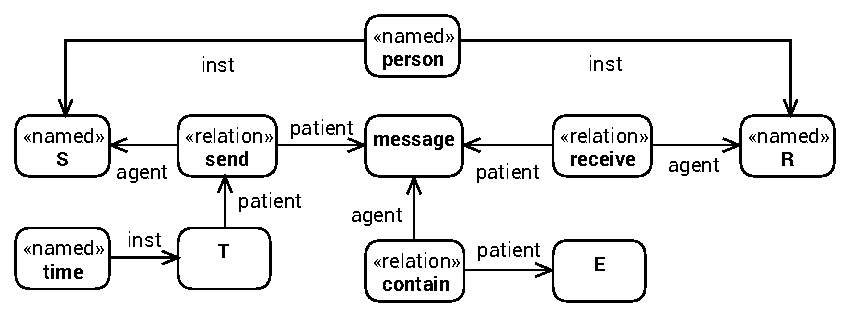
\includegraphics[scale=\cgScale]{gfx/text2kg/messageGraph.pdf}
		\end{align*}
		Die $patient(\text{contain}, E)$-Kante hat dabei den Wurzel-Möglichkeitskontext von $E$ als Ziel.
	\item \textbf{Konjunktion:}
		Der um Metadaten erweiterte Extraktionsgraph kann nun mit dem Wissensgraphen kombiniert werden.
		Hierfür werden lediglich die Knoten- und Kantenmengen vereinigt.
		Dies entspricht der logischen Konjunktion der durch beide Graphen repräsentierten Ausdrücke.
	\item \textbf{Koreferenzen:}
		Im Konjunktionsgraph befinden sich i.~d.~R. bekannte koreferente Konzepte.
		Um den Graphen zu vereinfachen und die Inferenz zu vereinfachen, sollten diese Konzepte zusammengefasst werden.
		Konkret handelt es sich hierbei um die NER-Klassen-Konzeptknoten (Person, Ort, Datum etc.), die latenten Konzepte und um die Knoten, die für $S$ und $R$ eingefügt wurden.
		Diese drei Arten von Knoten können bereits durch vorherige Nachrichten Teil des Wissensgraphen geworden sein und müssen beim Hinzukommen einer neuen Nachricht nicht erneut eingefügt werden.
\end{enumerate}

\subsection{Relationsinferenz mit PSL}%
\label{sec:text2kg:psl:inference}

Der Konjunktionsgraph wird nun als Eingabe für ein PSL-Programm verwendet, welches neue Relationen zwischen den Konzepten inferieren soll.
In diesem Abschnitt wird beschrieben, wie ein solches PSL-Programm aussehen kann.

\paragraph{PSL-Prädikate}
Im ersten Schritt müssen die verwendeten PSL-Prädikate definiert werden.
Hier bietet es sich an, die sechs Konzeptgraph-Relationen zu übernehmen.
Darüber hinaus müssen allerdings noch Prädikate für die Modellierung der Kontextstruktur definert werden.
\begin{enumerate}[noitemsep]
	\item $concept: \textbf{UUID}$: Markiert nicht latente Konzeptknoten.
	\item $concept_{latent}: \textbf{UUID}$: Markiert latente Konzeptknoten.
	\item $label: \textbf{UUID} \times \textbf{String}$: Aus der Ontologie übernommen.
	\item $named: \textbf{UUID}$: Aus der Ontologie übernommen.
	\item $inst: \textbf{UUID} \times \textbf{UUID}$: Aus der Ontologie übernommen.
	\item $relation: \textbf{UUID}$: Aus der Ontologie übernommen.
	\item $agent: \textbf{UUID} \times \textbf{UUID}$: Aus der Ontologie übernommen.
	\item $patient: \textbf{UUID} \times \textbf{UUID}$: Aus der Ontologie übernommen.
	\item $similar: \textbf{String} \times \textbf{String}$: Die Jaro-Ähnlichkeit der gegebenen Strings.
		Falls zwei Strings $A, B$ eine Distanz~$< 0.75$ haben, gilt jedoch $similar(A, B) = 0$.
	\item $context: \textbf{UUID}$: Markiert Kontexte.
	\item $possibility: \textbf{UUID}$: Markiert Möglichkeitskontexte.
	\item $negative: \textbf{UUID}$: Markiert negative Kontexte.
	\item $nest: \textbf{UUID} \times \textbf{UUID}$: Ordnet Kontexten ihre direkten Kindknoten zu.
	\item $nest_{indirect}: \textbf{UUID} \times \textbf{UUID}$: Ordnet jedem Kontext alle Knoten zu, die von seiner Kontextbox umschlossen sind.
\end{enumerate}
\edef\pslPredCount{\theenumi}

Bei $similar$ handelt es sich um ein sog.\ funktionales Prädikat.
Funktionale Prädikate werden intensional durch eine Funktion beschrieben und dürfen weder in der offenen Atommenge $\mathbb{O}$, noch in der geschlossenen Atommenge $\mathbb{C}$ vorkommen, da weder das Definieren noch das Inferieren von Grundatomen eines solchen Prädikates sinnvoll ist.
$similar$ wird verwendet, um die $label$-Ähnlichkeit von $named$-Konzepten bei der Inferenz berücksichtigen zu können.
Es wurde das Jaro-Ähnlichkeitsmaß gewählt, da es für Namen gute Ergebnisse liefert und sich zudem effizient berechnen lässt~\cite{Christen2006}, was aufgrund der zahlreichen Vergleiche, die im Rahmen einer Inferenz durchgeführt werden, wichtig ist.
Ähnlichkeitswerte~$< 0.75$ werden auf $0$ abgerundet, damit unähnliche $label$ bei der Inferenz gar nicht erst betrachtet werden.
Der Schwellwert $0.75$ wurde manuell gewählt~\tref{sec:conclusion:todo}.

\paragraph{Allgemeine PSL-Regeln}
Basierend auf der Semantik der PSL-Prädikate, lassen sich allgemeine PSL-Regeln definieren, die unabhängig von der Bedeutung einzelner Konzepte wahr sind.
Ein Teil dieser Regeln modelliert negative Priors und Transitivität.
Der Rest modelliert verschiedene Annahmen über die Struktur der Prädikate.
Konkret wird folgende Regelmenge verwendet:
\begin{itemize}
	\item \textbf{Regeln zur $inst$-Inferenz:}
	\begin{align*}
		0.2:\ & label(A, L_A) \land label(B, L_B) \land similar(L_A, L_B)  & \rulemark{rule:text2kg:inst:sim} \\
			& \land nest(C_A, A) \land nest_{indirect}(C_A, B) \land A \neq B \\
			& \land named(A) \land named(B) \rightarrow inst(A, B) \displaybreak[0]
		\intertext{Die Regel~\ruleref{rule:text2kg:inst:sim} modelliert die Annahme, dass zwischen zwei $named$-Konzepten $A, B$ mit ähnlichen Labeln u.~U.\ eine $inst(A, B)$-Beziehung besteht;
		Voraussetzung dafür ist, dass $B \leq A$ gilt.}
		0.1:\ & \lnot inst(A, B) & \rulemark{rule:text2kg:inst:prior} \displaybreak[0]\\[1ex]
		\infty:\ & inst(A, B) \land inst(B, C) \rightarrow inst(A, C) & \rulemark{rule:text2kg:inst:trans} \displaybreak[0]\\[1ex]
		\infty:\ & inst(A, B) \rightarrow \lnot inst(B, A) & \rulemark{rule:text2kg:inst:asym}\displaybreak[0]
		\intertext{\ruleref{rule:text2kg:inst:prior} beschreibt, dass $inst$ im Allgemeinen nicht gilt.
		Die Constraints \ruleref{rule:text2kg:inst:trans} und \ruleref{rule:text2kg:inst:asym} bilden die Transitivität und Asymmetrie von $inst$ ab.
	\item \textbf{Regeln zur $concept$-Inferenz:}}
		0.05:\ & concept_{latent}(A) \land inst(A, B) \rightarrow concept(A) & \rulemark{rule:text2kg:concept:hasinst} \\[1ex]
		0.5:\ & concept(A) \land concept_{latent}(B) \land inst(A, B) \rightarrow concept(B) & \rulemark{rule:text2kg:concept:isinst} \\[1ex]
		0.1:\ & \lnot concept(A) & \rulemark{rule:text2kg:concept:prior}
		\intertext{\ruleref{rule:text2kg:concept:hasinst} modelliert die Annahme, dass ein latentes Konzept mit mehreren Instanzen vermutlich ein tatsächliches Konzept ist.
		\ruleref{rule:text2kg:concept:isinst} beschreibt umgekehrt, dass ein latentes Konzept, das Instanz eines tatsächlichen Konzeptes ist, vermutlich ebenfalls ein tatsächliches Konzept ist.
	\item \textbf{Regeln zur $nest_{indirect}$-Inferenz:}}
		\infty:\ & nest(A, B) \rightarrow nest_{indirect}(A, B) & \rulemark{rule:text2kg:nest:dir} \\[1ex]
		\infty:\ & nest_{indirect}(A, B) \land nest(B, C) \rightarrow nest_{indirect}(A, C) & \rulemark{rule:text2kg:nest:trans}
		\intertext{Da nur $nest$-Relationen und keine $nest_{indirect}$-Relationen in der Eingabe vorhanden sind, müssen letztere mit \ruleref{rule:text2kg:nest:dir} und \ruleref{rule:text2kg:nest:trans} inferiert werden.
	\item \textbf{Geschlossene Prädikate:}}
		\infty:\ & \lnot named(A) & \rulemark{rule:text2kg:closed:named} \displaybreak[0]\\[1ex]
		\infty:\ & \lnot relation(A) & \rulemark{rule:text2kg:closed:relation} \displaybreak[0]\\[1ex]
		\infty:\ & \lnot nest(A) & \rulemark{rule:text2kg:closed:nest} \displaybreak[0]
		\intertext{Der Zweck dieser Priors ist es, zu verhindern, dass zusätzlich zu den $named$-, $relation$- und $nest$-Atomen des Konjuktionsgraphen weitere derartige Atome inferiert werden.
		Da bei der PSL-Inferenz keine NLP-Informationen zur Verfügung stehen, können diese Prädikate nämlich im Allgemeinen nicht sinnvoll inferiert werden und werden daher von der Inferenz ausgeschlossen.}
	\end{align*}%
\end{itemize}

\paragraph{Domänenspezifische PSL-Regeln}
Die allgemeinen Regeln sind nicht ausreichend, um aus einem gegebenen Konjunktionsgraphen relevante Erkenntnisse zu ziehen.
Hierfür ist domänenspezifisches Wissen und eine zugehörige Regelmenge notwendig.
Um das Grundprinzip zu veranschaulichen wird in dieser Arbeit eine sehr einfache domänenspezifische Regelmenge verwendet.
Abhängig vom betrachteten Datenset, sind für die Inferenz mit realen Kommunikationsdaten i.~d.~R. deutlich umfangreichere Regelmengen notwendig.

Die verwendeten domänenspezifischen Regeln führen zusätzlich zu den \pslPredCount\ allgemeinen PSL-Prädikaten weitere Prädikate ein, die zur Repräsentation von Zwischenergebnissen benutzt werden.
Diese zusätzlichen Prädikate sind nicht unbedingt notwendig, sondern vereinfachen lediglich die Regeldefinition.
Die folgenden domänenspezifischen Regeln werden verwendet:
\begin{align*}
	1:\ & context(ctx) \land patient(contain, ctx) \land agent(contain, msg) & \rulemark{rule:text2kg:message} \\
		& \land inst(\texttt{''concept\_contain''}, contain) \rightarrow {\color{blau}message}(ctx, msg) \displaybreak[0]\\[1ex]
	1:\ & {\color{blau}message}(ctx, msg) \land patient(send, msg) \land agent(send, sender) & \rulemark{rule:text2kg:sender} \\
		& \land inst(\texttt{''concept\_send''}, send) \rightarrow {\color{blau}sender}(ctx, sender) \displaybreak[0]\\[1ex]
	1:\ & {\color{blau}message}(ctx, msg) \land patient(receive, msg) \land agent(receive, receiver) & \rulemark{rule:text2kg:receiver} \\
		& \land inst(\texttt{''concept\_receive''}, receive) \rightarrow {\color{blau}receiver}(ctx, receiver) \displaybreak[0]\\[1ex]
	1:\ & nest_{indirect}(ctx, I) \land inst(\texttt{''concept\_I''}, I) & \rulemark{rule:text2kg:i} \\
		& \land {\color{blau}sender}(ctx, sender) \rightarrow inst(sender, I) \displaybreak[0]\\[1ex]
	1:\ & nest_{indirect}(ctx, you) \land inst(\texttt{''concept\_you''}, you) & \rulemark{rule:text2kg:you} \\
		& \land {\color{blau}receiver}(ctx, receiver) \rightarrow inst(receiver, you) \displaybreak[0]\\[1ex]
	1:\ & inst(\texttt{''concept\_uncombinable''}, x) \land inst(x, p_1) \land inst(x, p_2) & \rulemark{rule:text2kg:uncomb} \\
		& \land inst(p_1, y) \land inst(p_2, y) \land p_1 \neq p_2 \land \lnot inst(p_2, p_1) \rightarrow inst(p_1, p_2)
\end{align*}
\ruleref{rule:text2kg:message}, \ruleref{rule:text2kg:sender} und \ruleref{rule:text2kg:receiver} ordnen Nachrichten ihre Sender und Empfänger zu, was aufgrund der einheitlichen Repräsentation der Nachrichtenmetadaten im Konjunktionsgraphen eindeutig möglich ist.
\ruleref{rule:text2kg:i} und \ruleref{rule:text2kg:you} beschreiben, dass die Konzepte \textit{I} und \textit{you} innerhalb einer Nachricht auf den Sender bzw.\ den Empfänger dieser Nachricht verweisen.
Interessanter ist die Regel \ruleref{rule:text2kg:uncomb}.
Falls ein Konzept $y$ Instanz zweier Konzepte $p_1 \neq p_2$ ist, die wiederum Instanz eines \textit{uncombinable} Konzeptes $x$ sind, gilt entweder $inst(p_1, p_2)$ oder $inst(p_2, p_1)$.
Der Zweck dieser Regel wird im Kontext des im Folgenden beschriebenen domänenspezifischen Vorwissens deutlich.

\paragraph{Domänenspezifisches Vorwissen}
Damit die domänenspezifischen Regeln die gewünschten Ergebnisse liefern, müssen sie um domänenspezifisches Wissen ergänzt werden.
Dieses Wissen ist im Wesentlichen der Initialzustand des Wissensgraphen, bevor Nachrichten eingefügt wurden.
In dieser Arbeit wird der folgende initiale Wissensgraph verwendet:
\begin{align*}
	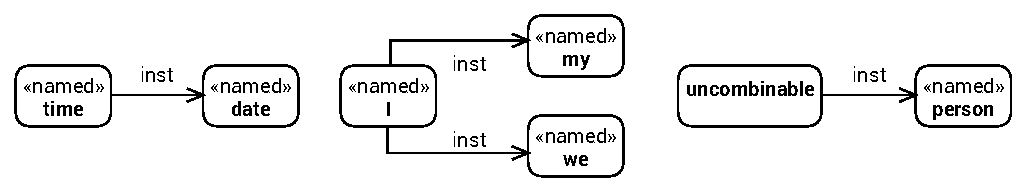
\includegraphics[scale=\cgScale]{gfx/text2kg/initialGraph.pdf}
\end{align*}\\
Für die Analyse von Nachrichten, die viel domänenspezifisches Wissen enthalten, ist offensichtlich eine wesentlich umfangreichere Wissensbasis erforderlich.
Hierfür könnten frei verfügbare semantische Netze, wie z.~B.\ WordNet~\cite{WordNet}, NELL~\cite{Carlson2010} oder YAGO~\cite{YAGO} verwendet werden.

Um das Grundprinzip des Konstruktionsverfahren zu illustrieren, ist ein kleiner initialer Wissensgraph allerdings vollkommen ausreichend.
Es sind im Wesentlichen drei Tatsachen kodiert:
Ein Datum ist eine spezielle Form der Zeitangabe, die Konzepte \textit{my} und \textit{we} schließen u.~a.\ das Konzept \textit{I} ein und Personen sind \textit{uncombinable}.
Letztere Relation wird verwendet, damit \ruleref{rule:text2kg:uncomb} für Personen gilt.
Falls also ein Konzept Instanz zweier Personen ist, muss eine dieser beiden Personen eine Instanz der anderen Person sein.
Anders formuliert bedeutet dies, dass ein Konzept nicht zugleich zwei verschiedene Personen $p_1 \neq p_2$ repräsentieren kann.
Die Eigenschaften $prop(p_1), prop(p_2)$ sind also nicht frei kombinierbar.

\paragraph{Wissensgraph-Konstruktion}
Die Wissensgraph-Konstruktion lässt sich nun als Inferenz mit dem PSL-Programm $R = \{ \ruleno{1}, \dots, \rulecurrent \}$ verstehen.
Die geschlossenen Grund\-atome $\mathbb{C}$ der Eingabe sind die Relationen im Konjunktionsgraphen, die keine offenen Grundatome in einer vorherigen PSL-Inferenz waren.
Wären zuvor inferierte Atome Teil von $\mathbb{C}$, könnten diese während der Inferenz nämlich nicht mehr aktualisiert werden, was z.~B. beim Einfügen von zusätzlicher Evidenz für eine bereits vorhandene Relation wichtig ist.
Als offene Grundatommenge $\mathbb{O}$ wird die Menge aller möglicher Relationen verwendet, die nicht in $\mathbb{C}$ liegen.
$\mathbb{O}$ kann und muss dabei nicht vollständig in den Speicher geladen werden.
Stattdessen wird eine sog.\ Lazy-Inference verwendet, d.~h.\ alle Atome in $\mathbb{O}$ werden erst dann instanziiert, wenn sie das erste Mal in einer Grundregel auftauchen.
Als Inferenzverfahren wird das in~\ref{sec:theory:psl:inference} vorgestellte ADMM-Verfahren benutzt.
BOCI konnte nicht benutzt werden, da es in seiner aktuellen Form erfordert, dass keine neuen Grundatome zwischen zwei Inferenzen hinzukommen;
beim Einfügen einer Nachricht gilt dies offensichtlich nicht.
Jede eingefügte Nachricht erfordert also eine vollständige ADMM-Inferenz.

Nach dem Ausführen von ADMM wird im letzten Schritt die Menge der inferierten Atome $\mathbb{O}$ als Menge von Konzeptgraph-Relationen interpretiert und zusammen mit $\mathbb{C}$ als neuer Wissensgraph verwendet.
Um die Graphgröße zu reduzieren werden dabei alle Atome mit einer Wahrscheinlichkeit $< 0.5$ verworfen.

\section{Implementation}%
\label{sec:text2kg:implementation}

Das in den vorherigen Abschnitten beschriebene Verfahren wurde im Rahmen dieser Arbeit prototypisch implementiert.
Bei der Wahl der hierfür verwandten Technologien wurde darauf Wert gelegt, dass eine möglichst nahtlose Integration der Komponenten möglich ist.
Sowohl CoreNLP~\cite{CoreNLP} als auch die PSL-Referenzimplementation~\cite{PSL} sind JVM-Bibliotheken.
Diese Arbeit wurde ebenfalls für die JVM implementiert, insbesondere weil es zu der JVM-basierten PSL-Referenzimplementation keine geeignete Alternative gibt und eine Reimplementation von PSL den Rahmen dieser Arbeit gesprengt hätte.

Als JVM-Sprache wurde Clojure gewählt, ein moderner Lisp-Dialekt.
Andere JVM-Sprachen, wie z.~B. Java, Scala oder Groovy, wurden ausgeschlossen, da sie sich während des Entwicklungsprozesses als hinderlich erwiesen haben.
Der Hauptgrund hierfür ist, dass CoreNLP bei der Initialisierung der Verarbeitungs-Pipeline diverse Modelle laden muss.
Abhängig von der benutzten Hardware dauert dies zwischen ca.\ 20 Sekunden und mehreren Minuten;
diese Wartezeiten sind ein stark verlangsamender Faktor, wenn sie nach jeder Code-Änderung auftreten.
Da Clojure ein Lisp ist, unterstützt es traditionsgemäß \textit{REPL Driven Development}.
Statt nach jeder Änderung die Anwendung neu zu starten und die Modelle erneut zu laden, kann so lediglich der geänderte Bytecode in den laufenden Prozess injiziert werden;
die geladenen Modelle bleiben dabei im Speicher und die Änderung kann ohne weitere Wartezeit getestet werden.
Durch die Wahl von Clojure konnte die Entwicklung deutlich beschleunigt werden.

Alle im folgenden Kapitel vorgestellten Tests wurden mit der entwickelten Referenzimplementation durchgeführt.
Die Rechte am Quelltext liegen bei der Firma Atos, er kann daher nicht frei verfügbar gemacht werden.
